% Compile from this directory: tectonic --keep-logs report.tex
% Or: pdflatex -interaction=nonstopmode -halt-on-error report.tex (twice)
\RequirePackage[T1]{fontenc}
\documentclass[conference,a4paper,10pt]{IEEEtran}
\usepackage[T1]{fontenc}
\usepackage{amsmath,amssymb}
\usepackage{graphicx}
\usepackage{cite}
\usepackage{xurl}
\usepackage[hidelinks]{hyperref}
\usepackage{microtype}
\usepackage{flushend}
\usepackage{needspace}
\usepackage{ragged2e}
\graphicspath{{../../figures/}}
\urlstyle{tt}
\def\UrlFont{\small\ttfamily}

% File paths may break at separators, never inside ordinary words or digits.
% Zero URL stretch avoids letterspacing when a path appears in a narrow column.
\newcommand{\filepath}[1]{\begingroup
  \def\UrlFont{\small\ttfamily}\Urlmuskip=0mu
  \def\UrlBreaks{\do\/\do\-\do\_\do\.}\def\UrlBigBreaks{\do\/}
  \nolinkurl{#1}\endgroup}

\emergencystretch=1em
\renewcommand{\IEEEkeywordsname}{Keywords}
\renewcommand{\dbltopfraction}{0.75}
\renewcommand{\textfraction}{0.15}
\setcounter{dbltopnumber}{2}
\title{Scalable K-means Clustering Using\\Hybrid MPI and OpenMP}
\author{\IEEEauthorblockN{Lai Xining}
\IEEEauthorblockA{DSA5208 Project 3\\5 November 2026}}
\hypersetup{pdftitle={Scalable K-means Clustering Using Hybrid MPI and OpenMP},pdfauthor={Lai Xining}}
\begin{document}
\maketitle
\thispagestyle{plain}
\pagestyle{plain}
\raggedbottom


\begin{abstract}

This project implements Lloyd-style K-means in C++17 as serial, MPI-only and hybrid MPI/OpenMP executables. Contiguous sample partitions distribute assignment work; replicated centroids are updated using two global reductions per iteration. Thread-private accumulators avoid synchronization in the inner assignment loop. Experiments on NUS Atlas compare strong scaling, weak scaling, rank/thread splits and input characteristics. For one million 16-dimensional samples, eight clusters and 50 fixed iterations, MPI at 12 active cores achieves $10.85\times$ loop speedup and 90.41\% strong efficiency relative to the serial baseline. The fastest tested genuinely multithreaded hybrid configuration, six ranks with two threads each, achieves $9.16\times$ speedup. With 250,000 samples per active core, 12-core weak efficiencies are 91.12\% for MPI and 93.51\% for hybrid, using different family baselines. All reported performance experiments are single-node CPU runs; they do not demonstrate inter-node scaling.

\end{abstract}

\begin{IEEEkeywords}\raggedright K-means, MPI, OpenMP, hybrid parallelism, strong scaling, weak scaling.\end{IEEEkeywords}

\section{Algorithm and motivation}

\noindent K-means groups vectors by minimizing the within-cluster sum of squared Euclidean distances (SSE):
\begin{equation}\mathrm{SSE}=\sum_{i=1}^{N}\lVert\mathbf{x}_i-\boldsymbol{\mu}_{\ell_i}\rVert_2^2.\end{equation}

The Lloyd iteration alternates assigning each sample to its nearest center and replacing each nonempty cluster center with the mean of its assigned samples \cite{lloyd}. It is relevant to data science as a clustering primitive and a controlled workload for studying repeated distance calculations and aggregation.

For N samples, d features and K centers, direct assignment takes $\mathcal{O}(NdK)$ work per iteration. Assignments can be evaluated independently only while centers are fixed. Every next iteration requires globally aggregated cluster sums and counts. This dependency makes the complete algorithm non-embarrassingly parallel.

The implementation stores double-precision, row-major data and selects K distinct seeded sample indices as initial centers. This is simple sample initialization, not k-means++. Exact distance ties select the lowest cluster index; empty clusters retain their old center. Normal execution stops when maximum Euclidean centroid displacement is at most the requested tolerance or the iteration limit is reached. Benchmarks instead use exactly 50 iterations to hold work constant. Final labels and SSE are recomputed using the returned centers. No global-optimum claim is made.

Synthetic input contains ten deterministic latent groups, independent of the requested K, with bounded noise. Global sample/feature indexing gives identical data across partitions. The study concerns computational behavior, not conclusions about a real population. No real dataset is used.

\section{Parallel design and tradeoffs}

MPI partitions contiguous rows with sizes differing by at most one. Synthetic input is generated locally, avoiding root distribution of the full benchmark dataset. Optional file input uses rank-zero loading and \path{MPI_Scatterv}, which can bottleneck root memory. Every rank stores all K centers, initialized consistently through a broadcast.

Within each rank, OpenMP statically partitions rows. Each thread accumulates private $Kd$ coordinate sums and K integer counts. These buffers remove data races and avoid atomics or critical sections for each sample. The main thread merges buffers in thread order; two \path{MPI_Allreduce} calls then combine double sums and integer counts. Allreduce makes the resulting statistics available to every rank \cite{allreduce}, so each rank can update its own identical center array. Separate reductions keep native numeric types and avoid a custom mixed-type reduction operation.

\path{MPI_THREAD_FUNNELED} is requested, the provided level is checked, and MPI calls occur outside OpenMP parallel regions. Threads do not independently call MPI. Static scheduling suits the approximately uniform direct-distance work per sample, but may be less suitable if future distance pruning creates irregular work.

Per-rank working memory is approximately $\mathcal{O}(Nd/P+TKd+Kd)$, excluding root file input and optional gathered diagnostics. P is the number of MPI ranks and T is threads per rank. Private buffers cost memory and must be cleared and merged every iteration; merging is serial within each rank. A new OpenMP parallel region is entered each iteration. These are potential hybrid overheads, not independently quantified causal explanations for the measured gap.

Increasing P reduces rows per rank but adds participants to collective synchronization. Increasing T reduces the number of MPI ranks needed for a fixed core count, while adding local thread coordination and merging. Neither choice guarantees better performance. All variants share numerical rules and most source code to make comparisons consistent; the serial executable uses neither MPI nor OpenMP, although it retains the common accumulator structure rather than being a separately hand-tuned baseline.

\section{Correctness and reproducibility}

The test suite compares small cases against a separately implemented Python Lloyd reference. Fixtures cover hand-computable updates, empty clusters, exact ties, identical samples, $K=1$, $K=N$, uneven partitions, ranks with zero rows, initialization, stopping behavior and invalid inputs. The earlier Atlas correctness job 1033975 reported 54 executable checks passing. Its complete raw run directory has now been downloaded: all 54 per-invocation evidence sets and the instrumented-test hash are retained. The formal-suite records below were also downloaded and directly checked.

Each formal job runs small numerical tests for all executable/rank/thread configurations against a serial reference on 103 rows, four features and five clusters. Labels must match; center comparisons use relative and absolute tolerance $1\times10^{-10}$, and SSE uses relative $1\times10^{-10}$ and absolute $1\times10^{-9}$. Every formal configuration passed. All 270 JSONL records, including warmups, were compared with their corresponding raw stdout records. Maximum relative SSE spread was approximately $5.97\times10^{-14}$ in strong scaling and $5.46\times10^{-14}$ within matched input shapes in the characteristics study. SSE is not compared across different-sized weak-scaling datasets.

Floating-point summation order changes with ranks and threads. Tolerance-based agreement supports correctness on tested inputs; bitwise reproducibility and identical convergence iteration counts are not promised. Successful tests are evidence, not a proof for all inputs.

\section{Atlas environment and measurement method}

All three successful formal jobs ran on the same allocated compute node. Recorded lscpu output identifies AMD EPYC 7R13, 96 guest-visible CPUs, two sockets, one thread per core and four NUMA nodes under KVM. Guest topology does not establish exclusive physical-host ownership. The software stack was GCC 7.3.0, OpenMPI 4.1.2, Python 3.8.5 and PBS Pro. Compilation used -O3 -std=c++17, with -fopenmp for the hybrid executable and \path{OMPI_SKIP_MPICXX=1} for MPI header compatibility.

The job environment purges modules, loads OpenMPI 4.1.2 and its GCC 7.3.0 dependency, then GMP 4.3.2 and MPFR 2.4.2. Python is invoked by absolute path without loading a Conda module. Explicit Atlas module search directories were added after an initial characteristics job could not locate OpenMPI on node 20. The patched job succeeded on node 25; node 20 was not retested.

Each formal job requested one node, 12 CPUs, 4 GB and 30 minutes in the parallel queue. Active cores are $P T$ and can be less than the 12 allocated cores. The launcher uses \path{slot:PE=T} mapping, core binding, no oversubscription and binding reports. \path{OMP_PLACES=cores}, \path{OMP_PROC_BIND=close} and \path{OMP_DYNAMIC=FALSE} are set. A separate probe checks per-thread affinity masks and distinct guest-visible cores for every $P,T$ pair before benchmarking. The scripts request \path{mpiprocs=ncpus}; nodefile slots should not generally be equated with CPU cores in other allocation layouts.

Each configuration has one excluded warmup and five measured repetitions. Configuration order is shuffled reproducibly in each sweep using seed 5208, reducing fixed-order bias. Reported values are medians; plotted ranges are measured minima and maxima, not confidence intervals. No outliers are removed. These are repeated runs within one allocation, not independent repeats across multiple nodes or days.

Strong scaling fixes $N=1{,}000{,}000$, $d=16$, $K=8$. Weak scaling fixes 250,000 rows per active core. Input characterization changes one of N, d or K at a time around the strong-scaling baseline. All use seed 42 and 50 fixed iterations.

Primary runtime is \path{loop_s}, the maximum iteration-loop duration over ranks. Application \path{end_to_end_s} excludes MPI initialization/finalization, launch and diagnostic output; the external timer includes launcher overhead. Component times are maxima over ranks and cannot be added as a decomposition of total time. Collective time can include waiting as well as communication.

For $C=PT$ active cores, strong speedup and efficiency are

\begin{equation}S(C)=\frac{\widetilde{t}_{\mathrm{serial,loop}}}{\widetilde{t}_{\mathrm{parallel,loop}}(C)},\qquad E(C)=\frac{S(C)}{C}.\end{equation}

Here $\widetilde{t}$ denotes the median runtime. Weak efficiency is

\begin{equation}E_{\mathrm{weak}}(C)=\frac{\widetilde{t}_{\mathrm{family}}(C_0)}{\widetilde{t}_{\mathrm{family}}(C)}.\end{equation}

The baseline is $C_0=1$ for MPI and $C_0=2$ for hybrid. The latter measures scaling from two cores, not absolute speed relative to serial.

Successful formal jobs were 1033995 (strong, 90 invocations), 1034060 (weak, 54) and 1034070 (characteristics, 126). PBS walltimes were 269, 215 and 463 seconds respectively, corresponding to 0.897, 0.717 and 1.543 allocated core-hours, or 3.157 in total. This excludes pilots, tests, builds and failed attempts. Requested limits total 18 core-hours for these three jobs. CPU-time accounting differs between final qstat and output epilogues; retain both and do not confuse either with allocated-core walltime.

\section{Strong scaling and rank/thread choices}

\begin{figure*}[t]

\centering

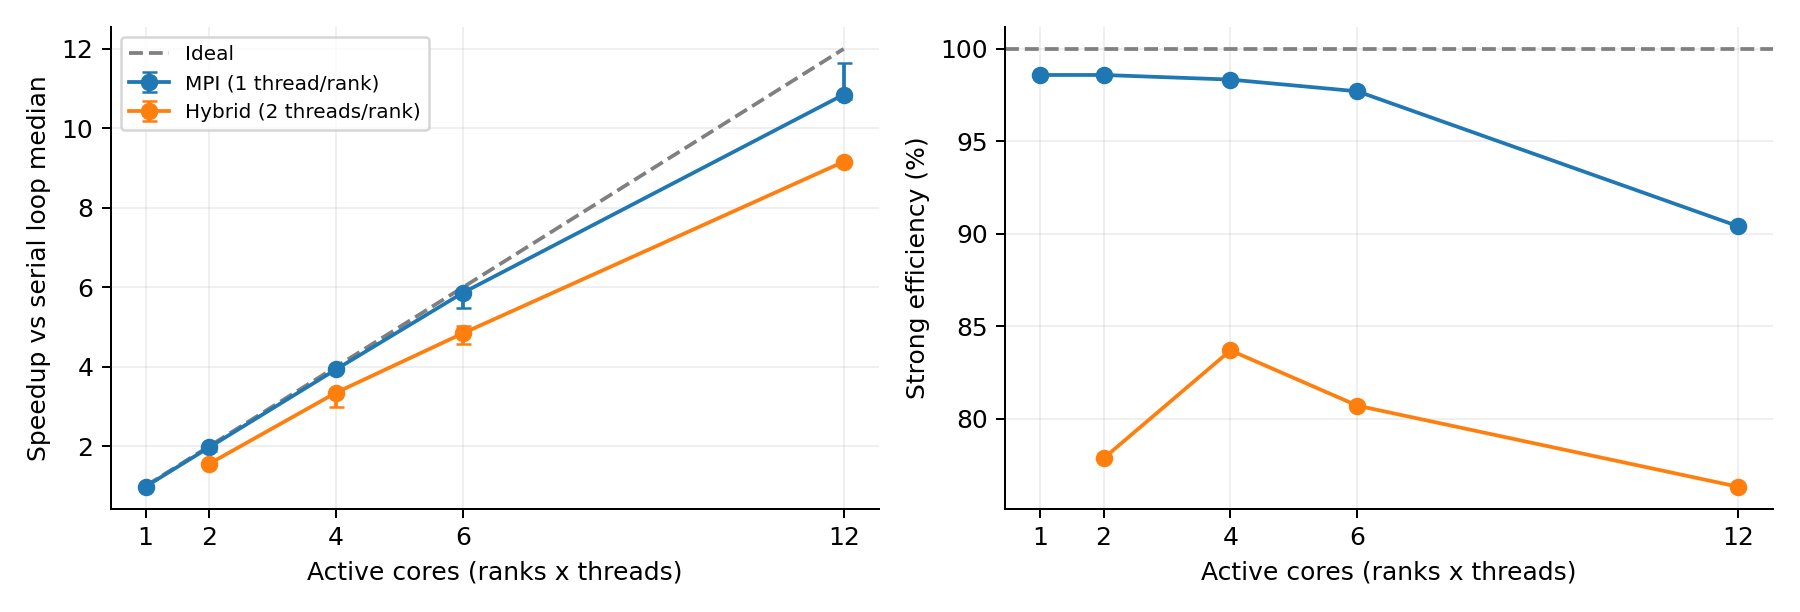
\includegraphics[width=0.96\textwidth]{strong_scaling.png}

\caption{Same $N,d,K$ and iteration count. Speedup error bars transform the observed parallel time range while holding the serial median fixed; they are not uncertainty intervals for the serial baseline. The hybrid curve keeps two threads per rank. Lines connect tested points only.}

\label{fig:1}

\end{figure*}

Figure~\ref{fig:1} summarizes strong scaling. Serial loop time is 3.656541 seconds. MPI $4\times1$ takes 0.929556 seconds ($3.934\times$ speedup, 98.34\% efficiency), MPI $6\times1$ takes 0.623724 seconds ($5.862\times$, 97.71\%), and MPI $12\times1$ takes 0.337016 seconds ($10.850\times$, 90.41\%). Efficiency falls at the largest tested core count. These results show useful parallel scaling but not perfectly proportional improvement.

\begin{figure*}[t]

\centering

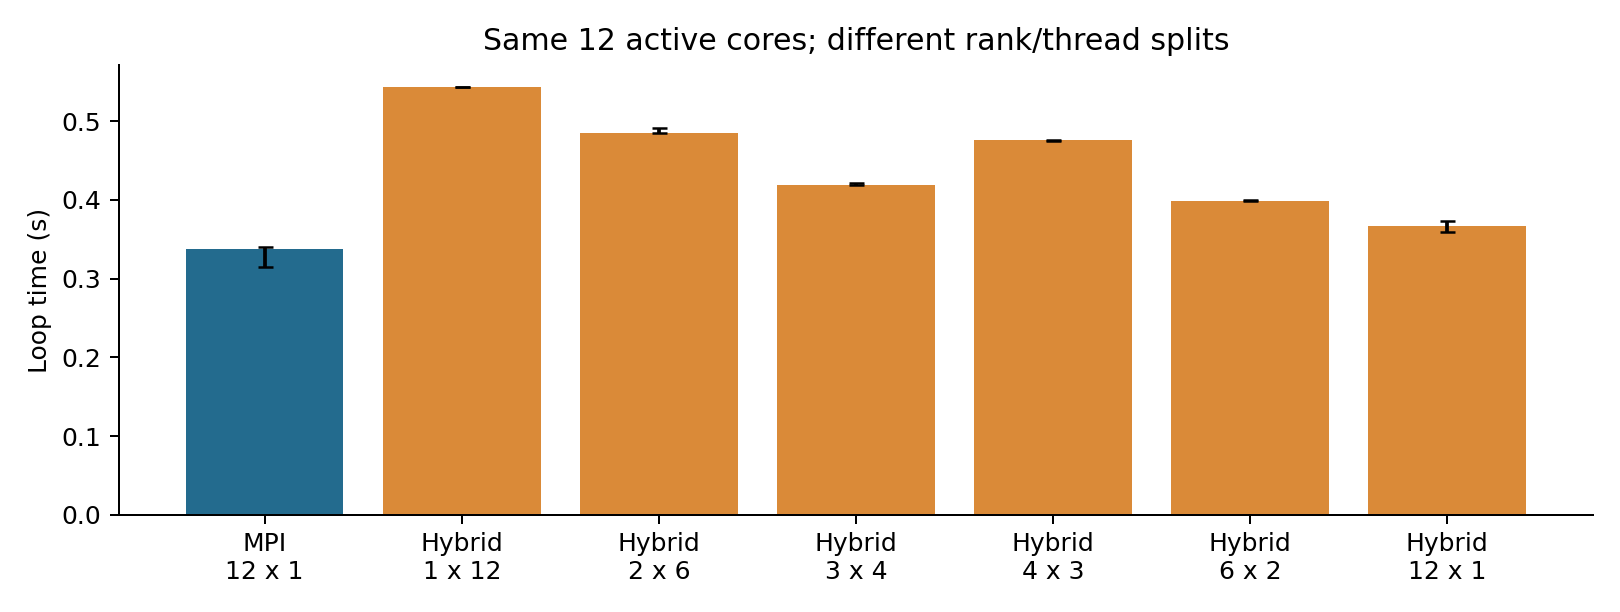
\includegraphics[width=0.96\textwidth]{rank_thread_split.png}

\caption{All configurations use 12 active cores; bars show median loop time and whiskers show minimum/maximum. Hybrid $12\times1$ is the OpenMP-enabled executable with one thread per rank, not a multithreaded run.}

\label{fig:2}

\end{figure*}

For the fixed-core comparison in Fig.~\ref{fig:2}, among hybrid configurations with $T>1$, $6\times2$ is fastest at 0.399183 seconds ($9.160\times$ speedup, 76.33\% efficiency). Hybrid $1\times12$ takes 0.543594 seconds, while hybrid $3\times4$ takes 0.418856 seconds and $4\times3$ takes 0.475753 seconds. The split matters even at fixed total cores. MPI $12\times1$ remains faster than every hybrid split tested. Thread coordination, merging, NUMA placement and shared-resource effects are plausible influences; this experiment does not isolate their individual contributions.

\section{Weak scaling and timing boundaries}

\begin{figure*}[t]

\centering

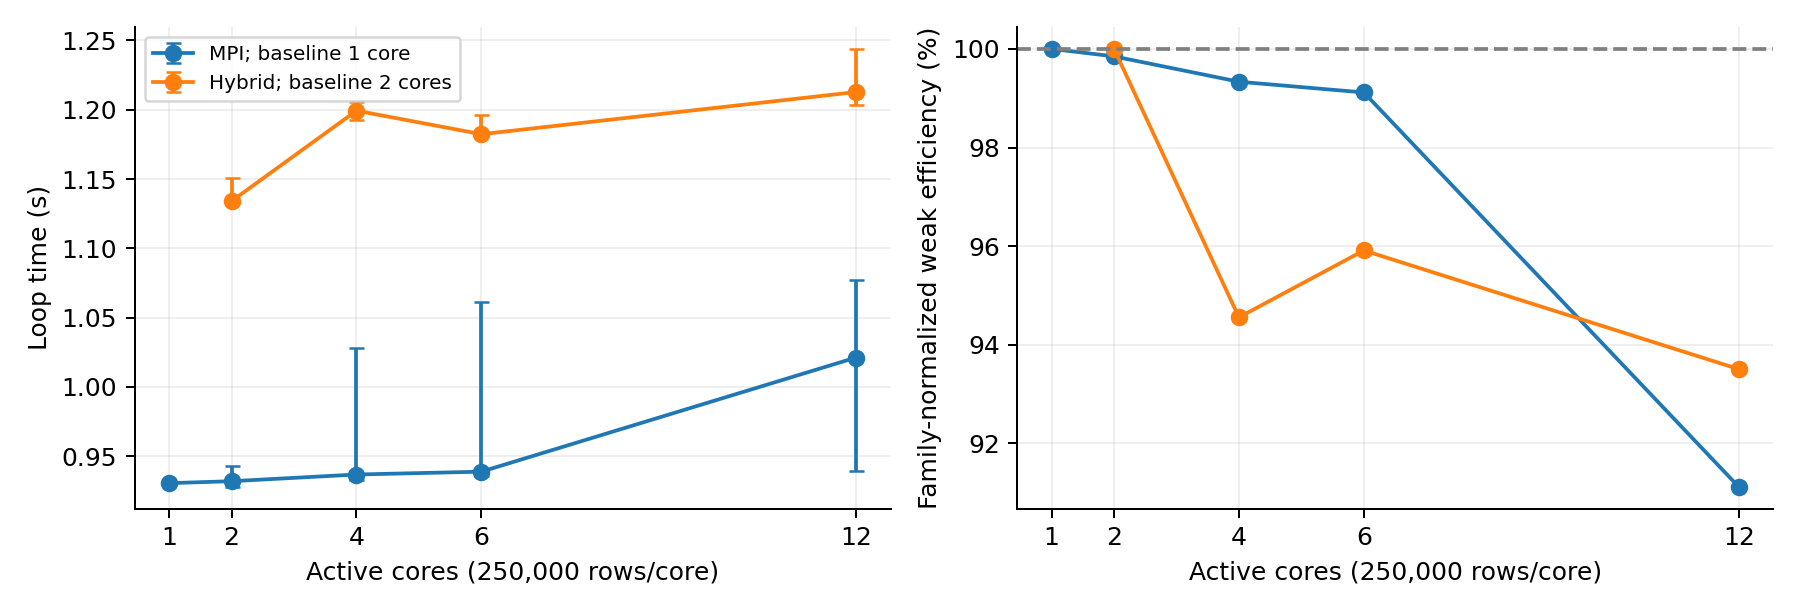
\includegraphics[width=0.96\textwidth]{weak_scaling.png}

\caption{Data grow from 250,000 rows on one MPI core to 3,000,000 rows on 12 cores. Hybrid starts at 500,000 rows on two cores. Each family uses its own smallest-core baseline. Runtime error bars are measured ranges.}

\label{fig:3}

\end{figure*}

In Fig.~\ref{fig:3}, MPI median loop time rises from 0.930485 seconds at one core to 1.021172 seconds at 12, giving 91.12\% weak efficiency. Hybrid rises from 1.134011 seconds at two cores to 1.212777 seconds at 12, giving 93.51\%. Higher hybrid normalized efficiency does not imply a faster implementation: MPI is faster in absolute time at 12 cores. MPI 12-core runs span 0.939346 to 1.077279 seconds, so variability is material to interpreting its median.

\begin{figure*}[t]

\centering

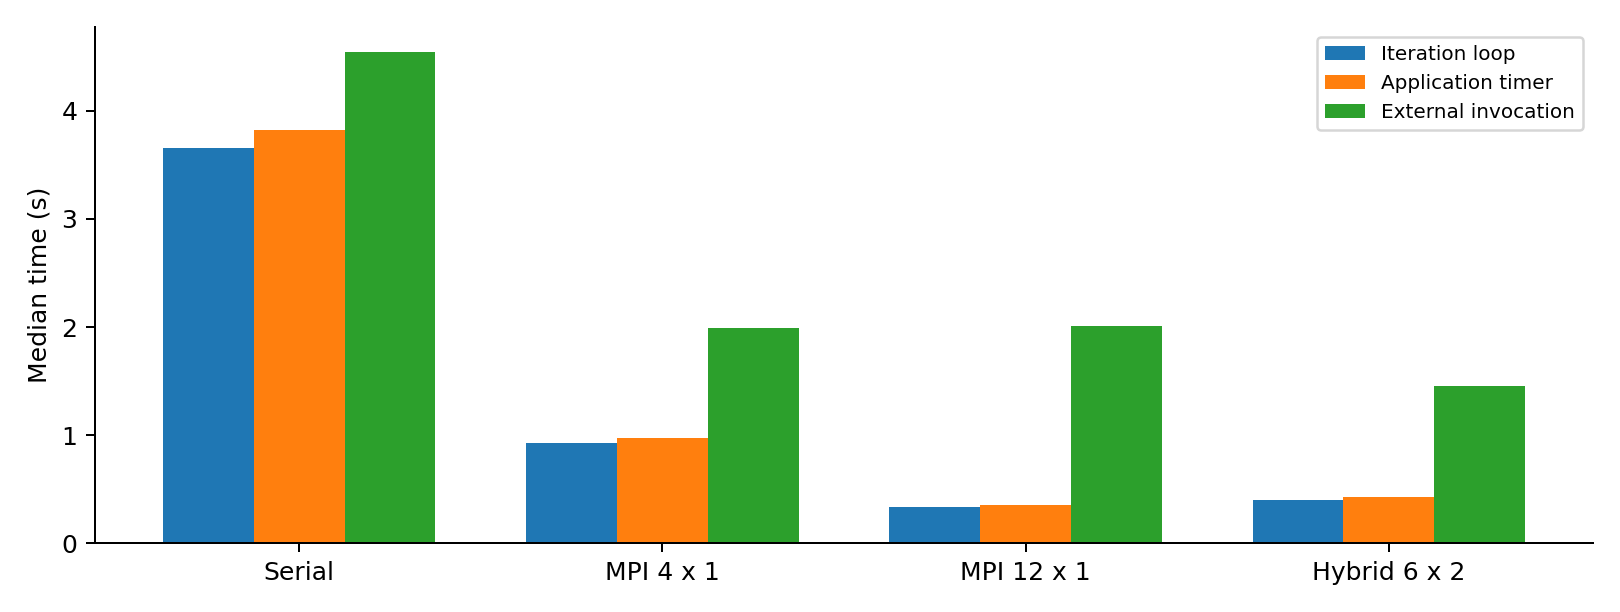
\includegraphics[width=0.96\textwidth]{timing_scope.png}

\caption{Strong-scaling median iteration-loop, application and external-invocation times. These measure different boundaries and must not be substituted for one another.}

\label{fig:4}

\end{figure*}

For the timing boundaries in Fig.~\ref{fig:4}, MPI $12\times1$ application time is 0.354353 seconds against serial 3.819063 seconds ($10.78\times$), whereas external invocation time is 2.008805 seconds against serial 4.549391 seconds ($2.26\times$). Hybrid $6\times2$ takes 0.424726 seconds at the application boundary ($8.99\times$) and 1.457985 seconds externally ($3.12\times$). Thus MPI wins the tested iteration-loop comparison, while hybrid $6\times2$ is faster than MPI $12\times1$ under external invocation timing. These external medians include launch overhead and variability; their difference does not identify a specific cause.

The loop speedups emphasize repeated Lloyd work. Setup, final assignment and launcher overhead reduce the benefit seen by a user timing an entire invocation. Fixed-iteration measurements also differ from time to convergence: configurations can perform different numbers of iterations under tolerance stopping because floating-point reductions differ. The report therefore does not claim the same speedup for convergence-based production workloads.

\Needspace{10\baselineskip}
\section{Input characteristics and limitations}

\begin{figure*}[t]

\centering

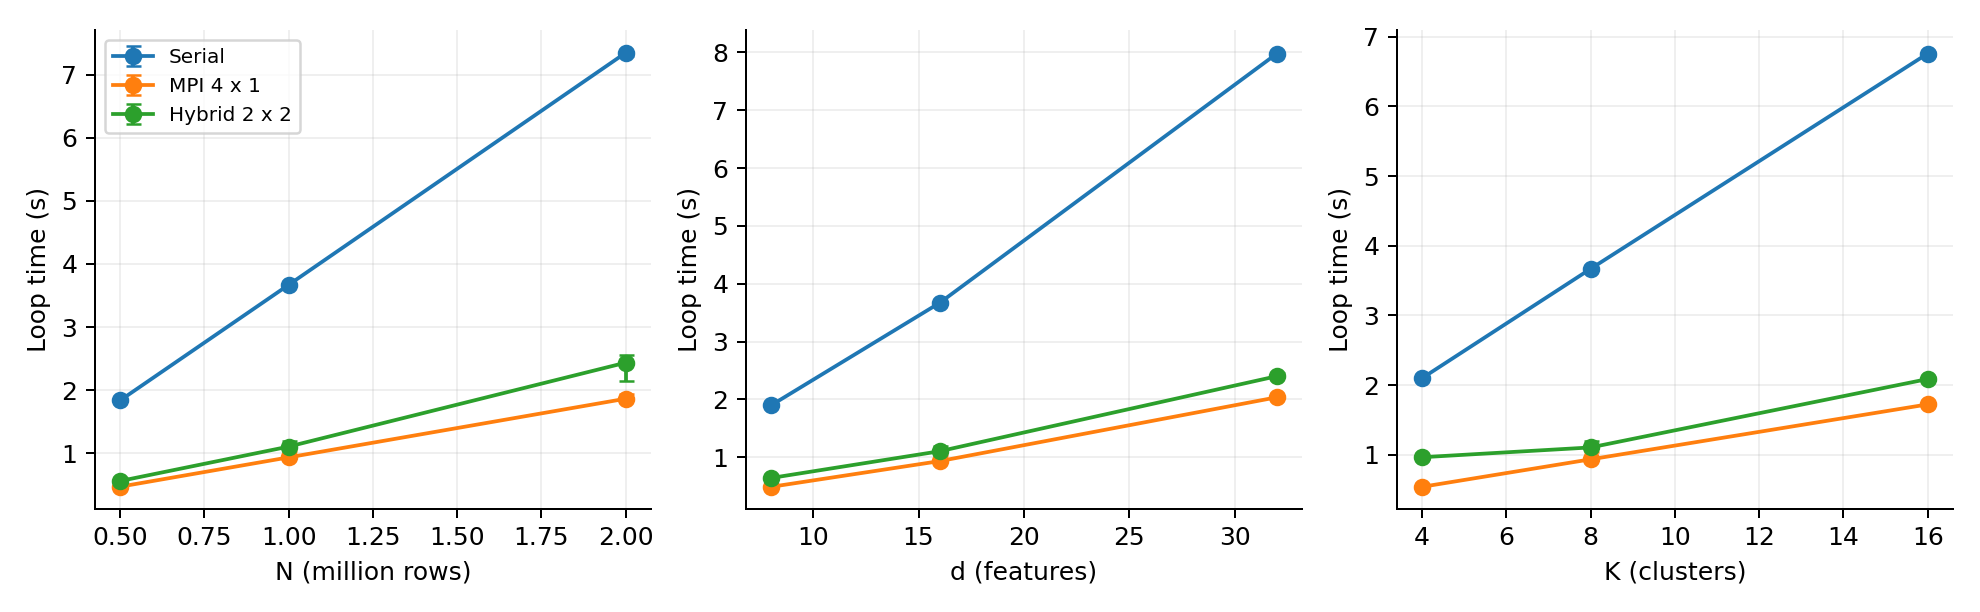
\includegraphics[width=0.96\textwidth]{input_characteristics.png}

\caption{One input parameter varies at a time; all other parameters remain at $N=1{,}000{,}000$, $d=16$, $K=8$. Each point is a five-run median with minimum/maximum whiskers. MPI uses $4\times1$ and hybrid $2\times2$, both four active cores; serial uses one.}

\label{fig:5}

\end{figure*}

For the input comparison in Fig.~\ref{fig:5}, at the baseline shape, serial, MPI and hybrid times are 3.668579, 0.933281 and 1.103982 seconds. Doubling N to two million gives 7.348370, 1.863028 and 2.434704 seconds. Serial and MPI scale almost proportionally with N; hybrid shows more variation, with its largest-N runs spanning 2.149055 to 2.560071 seconds.


Doubling d from 16 to 32 gives serial time 7.976496 seconds, about $2.17\times$ the baseline. Doubling K from 8 to 16 gives 6.759070 seconds, about $1.84\times$. These trends broadly match direct assignment's $\mathcal{O}(NdK)$ work, but finite overheads and machine behavior prevent exact proportionality. MPI $4\times1$ outperforms hybrid $2\times2$ for all seven tested shapes. Each speedup comparison must use the serial baseline for the same shape within this job, rather than reusing the earlier strong-scaling baseline.

No real-data interpretation is offered: synthetic data control workload size, and latent group count is not inferred from the requested K. Only one seed and a limited input range were benchmarked. No inter-node execution, GPU implementation, network scaling, parallel file reader or k-means++ initialization was tested. The conservative $Nd\leq\mathrm{INT\_MAX}$ guard limits MPI counts. Replicated centers, root file loading and thread-private buffer size limit large cases. Hardware counters were not collected, so bandwidth/cache explanations remain hypotheses.

\section{Conclusion}

The implementation demonstrates correct tested behavior and useful single-node MPI and MPI/OpenMP scaling on Atlas. Twelve-rank MPI reaches $10.85\times$ loop speedup, while the best tested multithreaded hybrid split reaches $9.16\times$. Weak scaling remains above 91\% at the largest tested scale using family-specific baselines. The main practical lesson is to measure rank/thread splits and timing boundaries rather than assuming hybrid execution is automatically faster. Further work should validate inter-node placement and transport, repeat on additional allocations, and profile thread coordination and memory locality before changing the algorithm.

\section{Reproduction and evidence}

\begingroup
\RaggedRight
\setlength{\parindent}{1em}
The source is available in the public \href{https://github.com/carus7749/parallel-kmeans-mpi-openmp}{GitHub repository}. The source package includes the C++ implementation, header files, build configuration, correctness tests, Atlas PBS scripts, environment initialization, an affinity probe, the experiment runner, and reproducibility documentation. The README documents build commands, command-line arguments and input format. Each Atlas job snapshots source, hashes files, compiles within its PBS allocation and preserves stdout/stderr, commands, node topology, environment, scheduler information and exit status. No computational workload was run by the assistant on a login node.

The complete measurement records for strong scaling, weak scaling, and input characterization are included in the accompanying source package, together with provenance, SHA256 identifiers and verification notes. The supplied plotting script regenerates all figures with Python, matplotlib and numpy. The report's IEEEtran LaTeX source and compilation instructions are included; exact file locations are provided in the README and supporting documentation. Nine downloaded run directories, including two failed attempts, are preserved in a separate evidence ZIP. Source and binary SHA256 manifests were checked; the instrumented correctness test is verified against its dedicated hash. The submissions directory is included, with job-ID records and final scheduler records for all nine jobs. Each final scheduler state is F and its exit status matches the run-directory exit code.
\par
\endgroup

\section*{AI Usage Disclosure}

OpenAI Codex was used extensively as an assistant throughout this project, including implementation, testing, debugging, performance analysis, visualization, and report preparation. The HPC experiments were conducted on NUS Atlas, and all reported performance results are based on actual measurements rather than generated estimates.

\begin{thebibliography}{2}
\RaggedRight
\Urlmuskip=0mu

\bibitem{lloyd} S. P. Lloyd, ``Least squares quantization in PCM,\textquotedblright\ \emph{IEEE Transactions on Information Theory}, vol. 28, no. 2, pp. 129--137, 1982. doi: \nolinkurl{10.1109/TIT.1982.1056489}.

\bibitem{allreduce} Open MPI Project, ``MPI\_Allreduce manual,\textquotedblright\ Open MPI 4.1 documentation family (web page currently labeled 4.1.8; experimental runtime was 4.1.2). [Online]. Available: \url{https://www.open-mpi.org/doc/v4.1/man3/MPI_Allreduce.3.php}

\end{thebibliography}

\end{document}
